\section{Data and endpoint definitions}
\label{sec:endpoints}
\label{sec:data-endpoints}

The three expansion histories compared in this paper were obtained
separately, before any comparison was made. Each is fixed: no
endpoint is refit, retuned, or extended anywhere in this analysis.
All headline values resolve through generated macros to the fixed
artifacts cited below. Symbols are defined once in the nomenclature
table (Table~\ref{tab:nomenclature}); throughout the main text,
R is the distance-compatible endpoint, C1 and C2 are the two
Planck-compatible endpoints, and the order-3 representation is the selected compact
reconstruction basis.

\begin{table}[!htbp]
  \centering
  \caption{Nomenclature: symbols used in the main analysis.}
  \label{tab:nomenclature}
  \begin{tabularx}{\linewidth}{lXXX}
    \toprule
    Symbol & Meaning & How obtained & Used for \\
    \midrule
    $R$ & distance-sector endpoint &
      fixed distance-sector endpoint & reference deformation \\
    $C_{1}$ & Planck-calibrated reference &
      Planck TT/TE/EE calibrated CAMB reference & CMB reference \\
    $C_{2}$ & secondary Planck-calibrated reference &
      separately implemented Planck/CAMB reference & sensitivity reference \\
    $\Delta_{1}$ & $\ln H_{R}(z)-\ln H_{C_{1}}(z)$ &
      derived & comparison \\
    $\Delta_{2}$ & $\ln H_{R}(z)-\ln H_{C_{2}}(z)$ &
      derived & comparison \\
    $\Delta_{C}$ & $\ln H_{C_{1}}(z)-\ln H_{C_{2}}(z)$ &
      derived & reference spread \\
    $K_{H}$ & overall amplitude of the reconstruction map &
      fitted (reconstruction coordinate) & compact representation \\
    $c_{j}$ & Legendre shape coefficients ($j=0,1,2$) &
      fitted (reconstruction coordinates) & compact representation \\
    $m=3$ & order-3 reconstruction &
      CV-selected & compact representation \\
    $\epsilon$ & reciprocity parameter &
      profiled & diagnostic only \\
    \bottomrule
  \end{tabularx}
\end{table}


\subsection{Distance-compatible endpoint R}
\label{sec:endpoint-r}

R is the fixed phenomenological distance-sector endpoint used in this comparison. It reaches $H_0=72.80$~km~s$^{-1}$~Mpc$^{-1}$, carries $r_d=135.39$~Mpc, and provides the low-redshift distance-sector reference history. The
compressed distance prior \citep{Chen2019} used during endpoint
discovery was validated only for conventional late-time models; it did
not validate the $r_{d}=135.39$~Mpc early-universe physics.

Concretely, R is the smooth low-redshift reference history
(pinned in
\path{paper/evidence/endpoints/endpoint_manifest.json}).
It reaches $H_{0}=\DistanceHZero$\kmsMpc{} with
$r_{d}=135.39$~Mpc and fits the DESI DR2 and Pantheon+SH0ES distance
sector. Nothing in Sections~\ref{sec:model-selection} or
\ref{sec:reference-sensitivity} depends on the history of how R was found.

\subsection{CMB-compatible endpoint C1}
\label{sec:endpoint-c1}

C1 is a Planck TT/TE/EE-compatible reference background with
$H_{0}=\CmbOneHZero$\kmsMpc{} and
$r_{\mathrm{drag}}=147.15$~Mpc, produced with the stated
CAMB/likelihood configuration.
No distance-sector parameter, table, or likelihood entered its construction.

\subsection{Secondary Planck-compatible reference C2}
\label{sec:endpoint-c2}

C2 is a secondary Planck-compatible $\Lambda$CDM reference with
$H_{0}=\CmbTwoHZero$\kmsMpc{}, used only as a reference-sensitivity
check, evaluated through its own Planck
likelihood. It shares the
Planck sky with C1 and uses nearly the same $\Lambda$CDM background
family with its own parameter choices and calibration route, so it
cannot provide independent cosmological confirmation. C1
and C2 are separately implemented in pipeline/model space, not
statistically independent in data space; both use Planck
information. Table~\ref{tab:endpoint-construction} compares the two
constructions row by row.

\subsection{Common observable representation}
\label{sec:endpoint-repr}

All three endpoints are compared on one common uniform-$u$ grid of
2000 nodes spanning $0 \le z \le 2.33$
(\path{paper/evidence/endpoints/endpoint_redshift.json}). The
difference fields
\[
\Delta_{1}(z) \equiv \ln H_{R}(z)-\ln H_{C_{1}}(z), \qquad
\Delta_{2}(z) \equiv \ln H_{R}(z)-\ln H_{C_{2}}(z), \qquad
\Delta_{C}(z) \equiv \ln H_{C_{1}}(z)-\ln H_{C_{2}}(z)
\]
are evaluated on that grid and fixed in
\path{paper/evidence/reference_sensitivity/difference_fields.npz}. The
constrained domain is $z \le 1.8$, covering all non-Ly$\alpha$ DESI
blocks; the Ly$\alpha$ anchor at $z=2.33$ tests the continuation law,
not the low-redshift deformation
(\path{paper/evidence/reference_sensitivity/domain_split.json}).

\begin{figure}[!htbp]
  \centering
  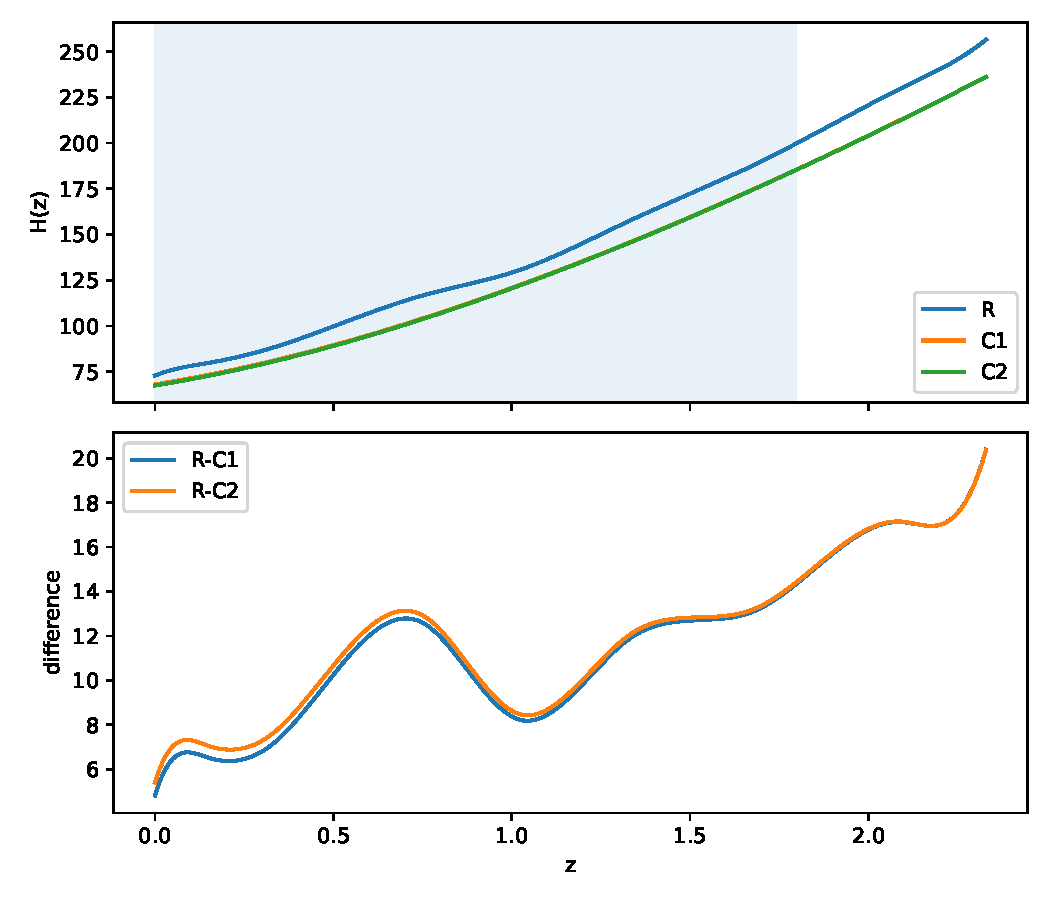
\includegraphics[width=0.9\linewidth]{figures/generated/overview_fig1_endpoints}
  \caption{Fixed endpoint overview (no fits in this figure). Top: the
  three fixed histories $H_{R},H_{C_{1}},H_{C_{2}}$; C1 and C2 nearly
  overlap in the upper panel and distinct line styles are used to keep
  both visible. Bottom: their
  logarithmic differences $\Delta_{1},\Delta_{2},\Delta_{C}$; across
  the constrained bins the RMS difference between C1 and C2 is approximately 1\% to 8\% of
  the corresponding RMS difference between R and either Planck reference.
  Shading marks the constrained domain $z\le1.8$; the dotted line
  marks the Ly$\alpha$ continuation test at $z=2.33$.}
  \label{fig:endpoint-overview}
\end{figure}

\subsection{Endpoint acoustic calibration}
\label{sec:calibration}

Each endpoint carries its own acoustic ruler, traced to fixed
artifacts in the endpoint calibration contract
(\path{paper/evidence/endpoints/calibration_contract.json}). Boltzmann
rulers are computed with CAMB \citep{Lewis2000}:

\begin{table}[!htbp]
  \centering
  \caption{Endpoint acoustic calibration: every endpoint's ruler.
  The compressed distance prior \citep{Chen2019} did not validate
  nonstandard early-universe physics for R.}
  \label{tab:calibration}
  \begin{tabular}{lllll}
    \toprule
    Endpoint & $r_{d}$ [Mpc] & $r_{s}$ [Mpc] &
      Fixed or recomputed? & Source \\
    \midrule
    R & 135.39 & --- (not used) &
      fixed (pinned control fit) & control fit \\
    C1 & 147.15 & 144.50 &
      recomputed (CAMB stage-0) & stage-0 background \\
    C2 & 147.11 & 144.45 &
      recomputed (CAMB baseline) & baseline acoustic \\
    \bottomrule
  \end{tabular}
\end{table}

R uses an early-ruler value different from C1/C2; this ruler
difference is part of the measured endpoint separation, not a shared
calibration. The R ruler is roughly $0.92$ of either CMB ruler, an
$\sim8\%$ smaller ruler. This is a property of the phenomenological
distance endpoint, not a demonstrated physical sound horizon: R's
$r_{d}=135.39$~Mpc is a phenomenological endpoint value and is not
validated as early-universe physics. The compressed Planck distance
prior \citep{Chen2019} was validated only for conventional
$\Lambda$CDM, $w$CDM, and CPL models and cannot by itself validate
such nonstandard pre-recombination physics; no BBN viability is
claimed (no BBN fit is performed). The BAO forward model is endpoint-specific:
\begin{equation}
  D_{M}/r_{d},\qquad D_{H}/r_{d},\qquad D_{V}/r_{d},
  \label{eq:bao-forward}
\end{equation}
evaluated with each endpoint's own ruler from
Table~\ref{tab:calibration}.

\begin{table}[!htbp]
  \centering
  \caption{Endpoint construction comparison: C1 versus C2.}
  \label{tab:endpoint-construction}
  {\small
  \begin{tabularx}{\linewidth}{lXX}
    \toprule
     & C1 & C2 \\
    \midrule
    Underlying CMB observations & Planck TT/TE/EE & Planck TT/TE/EE \\
    Boltzmann code & CAMB 2.0.4 & CAMB (baseline pipeline) \\
    Likelihood implementation & Planck TT/TE/EE likelihood (CAMB-based) &
      stock baseline Planck likelihood \\
    Cosmological parameterization & flat $\Lambda$CDM stage-0 &
      flat $\Lambda$CDM \\
    Primordial spectrum parameterization & power-law tilt &
      power-law tilt, $n_{s}=0.965$ \\
    Optimizer/sampler & background tuning (stage-0) &
      fixed-parameter baseline with spectral parity \\
    Background extraction & frozen CAMB table &
      CAMB-sampled $H(z)$ table \\
    $H_{0}$ [km\,s$^{-1}$\,Mpc$^{-1}$] & 67.99 & 67.4 \\
    $\Omega_{m}$ & 0.3075 & 0.3134 \\
    $r_{d}$ [Mpc] & 147.15 & 147.11 \\
    $r_{s}$ [Mpc] & 144.50 & 144.45 \\
    \bottomrule
  \end{tabularx}
  }
\end{table}

C1 and C2 are separately implemented in pipeline/model space,
not statistically independent in data space; both use Planck
information.

